\section{RESULT}
\subsection{Path traversal by the first robot}
From the initial position, the first robot began to traverse the maze and the required decisions at the junctions were taken on the basis of the priorities  provided by our left wall following algorithm and subsequently, the first robot traveled the entire maze and ultimately the target was detected.\\
The path followed by the robot is shown in the figure below: 
\begin{figure}[h]
\center
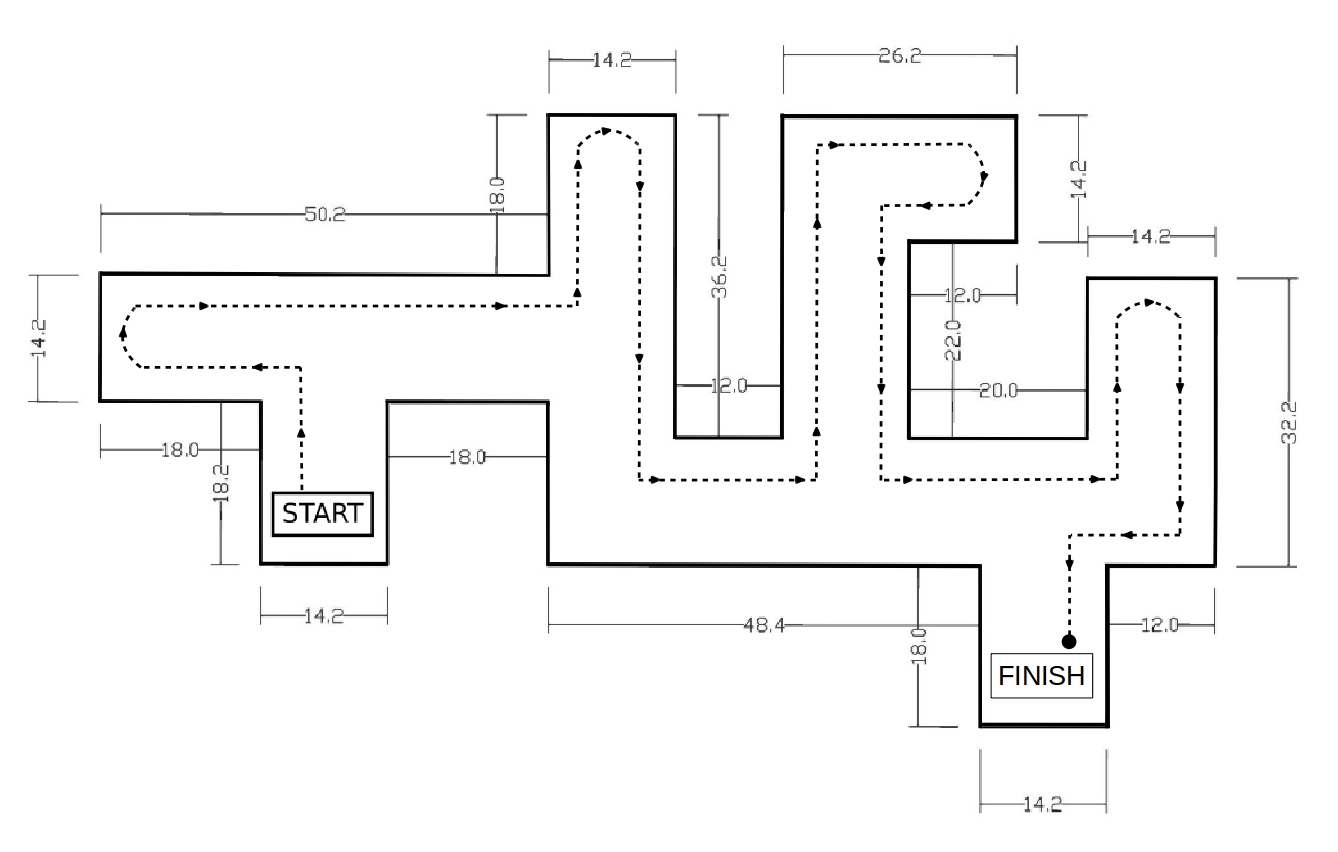
\includegraphics[scale=0.3]{mazetraverse_newnew.jpg} 
\caption{The path followed by the first robot}
\end{figure}
\subsection{Target Detection}
Eventually, the final target for the first robot to detect was chosen to be smoke.  The travelling robot does not know the location of the target which was present somewhere in the maze and subsequently detected the target using MQ-2 gas sensor which was implemented in the robot. \\
MQ-2 Gas Sensor works on the principle “The greater the gas concentration, the greater the output voltage" .Thus, the sensor analog output voltage was read and when it reached/crossed a certain threshold, the target detection decision was taken as positive and subsequently the first robot was stopped for any locomotion thereafter.
\begin{figure}[h]
\center
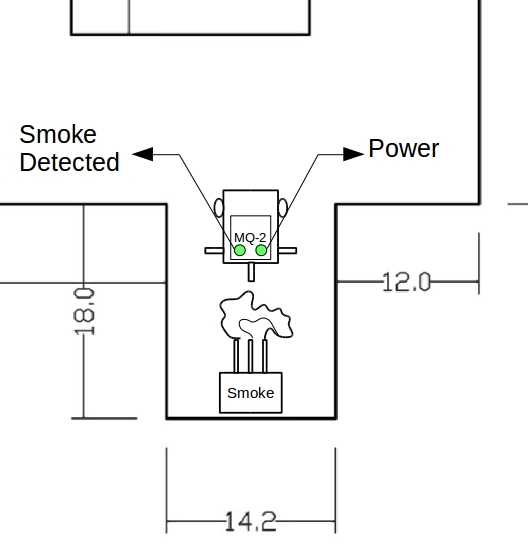
\includegraphics[scale=0.5]{part4_1_final.jpg} 
\caption{Target Detection by the first robot through MQ-2 Smoke Sensor}
\end{figure}
\subsection{Bluetooth Communication}
Both the LEDs of the master and slave setup HC-05 blinked at the rate of two fast blinks every two seconds. This indicated that both the master and slave modules were paired with each other.\\
The decisions taken at the junctions were then decode and were sent to the second robot via Bluetooth.\\ 
Thus, based upon the decoded message, the second robot traversed the maze in the shortest path possible. \\
The decisions made by the first robot at the junctions is shown in the figure below:\\
\newpage
\begin{figure}[h]
\center
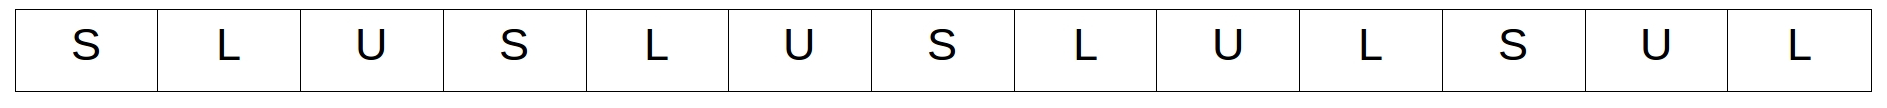
\includegraphics[scale=0.25]{packet_new.jpg} 
\caption{The decisions taken at the various junctions in the above given maze}
\end{figure}
\justify The above decisions were then decoded and was sent to the second robot via the Bluetooth module for traversing the maze in the shortest path possible.\\
\justify The decoded decisions are shown in the table below:
\begin{table}[h]
\begin{center}
\begin{tabular}{ |c|c|c|c|c| }
\hline 
S&R&R&S&R\\
\hline
\end{tabular}
\caption{The decoded decisions sent to the second robot}
\end{center}
\end{table}
\begin{table}[h]
\begin{center}
\begin{tabular}{ |c|c|c|c|c| }
\hline 
S&STRAIGHT\\
\hline 
R&RIGHT\\
\hline 
L&LEFT \\
\hline 
U&U-TURN\\
\hline
\end{tabular}
\caption{S,R,L,U Notations}
\end{center}
\end{table}
\subsection{Path traversal by the second robot}
The second robot received the information/decision from the first robot and started traversing the maze. The junction in the maze was detected by a set of IR Sensors similar to that on the first robot.  Upon the arrival of the junction ,  the second robot took the desired decision that led the robot through the shortest path to the target.\\
The path followed by the second robot is shown in the figure below:
\newpage
\begin{figure}[h]
\center
 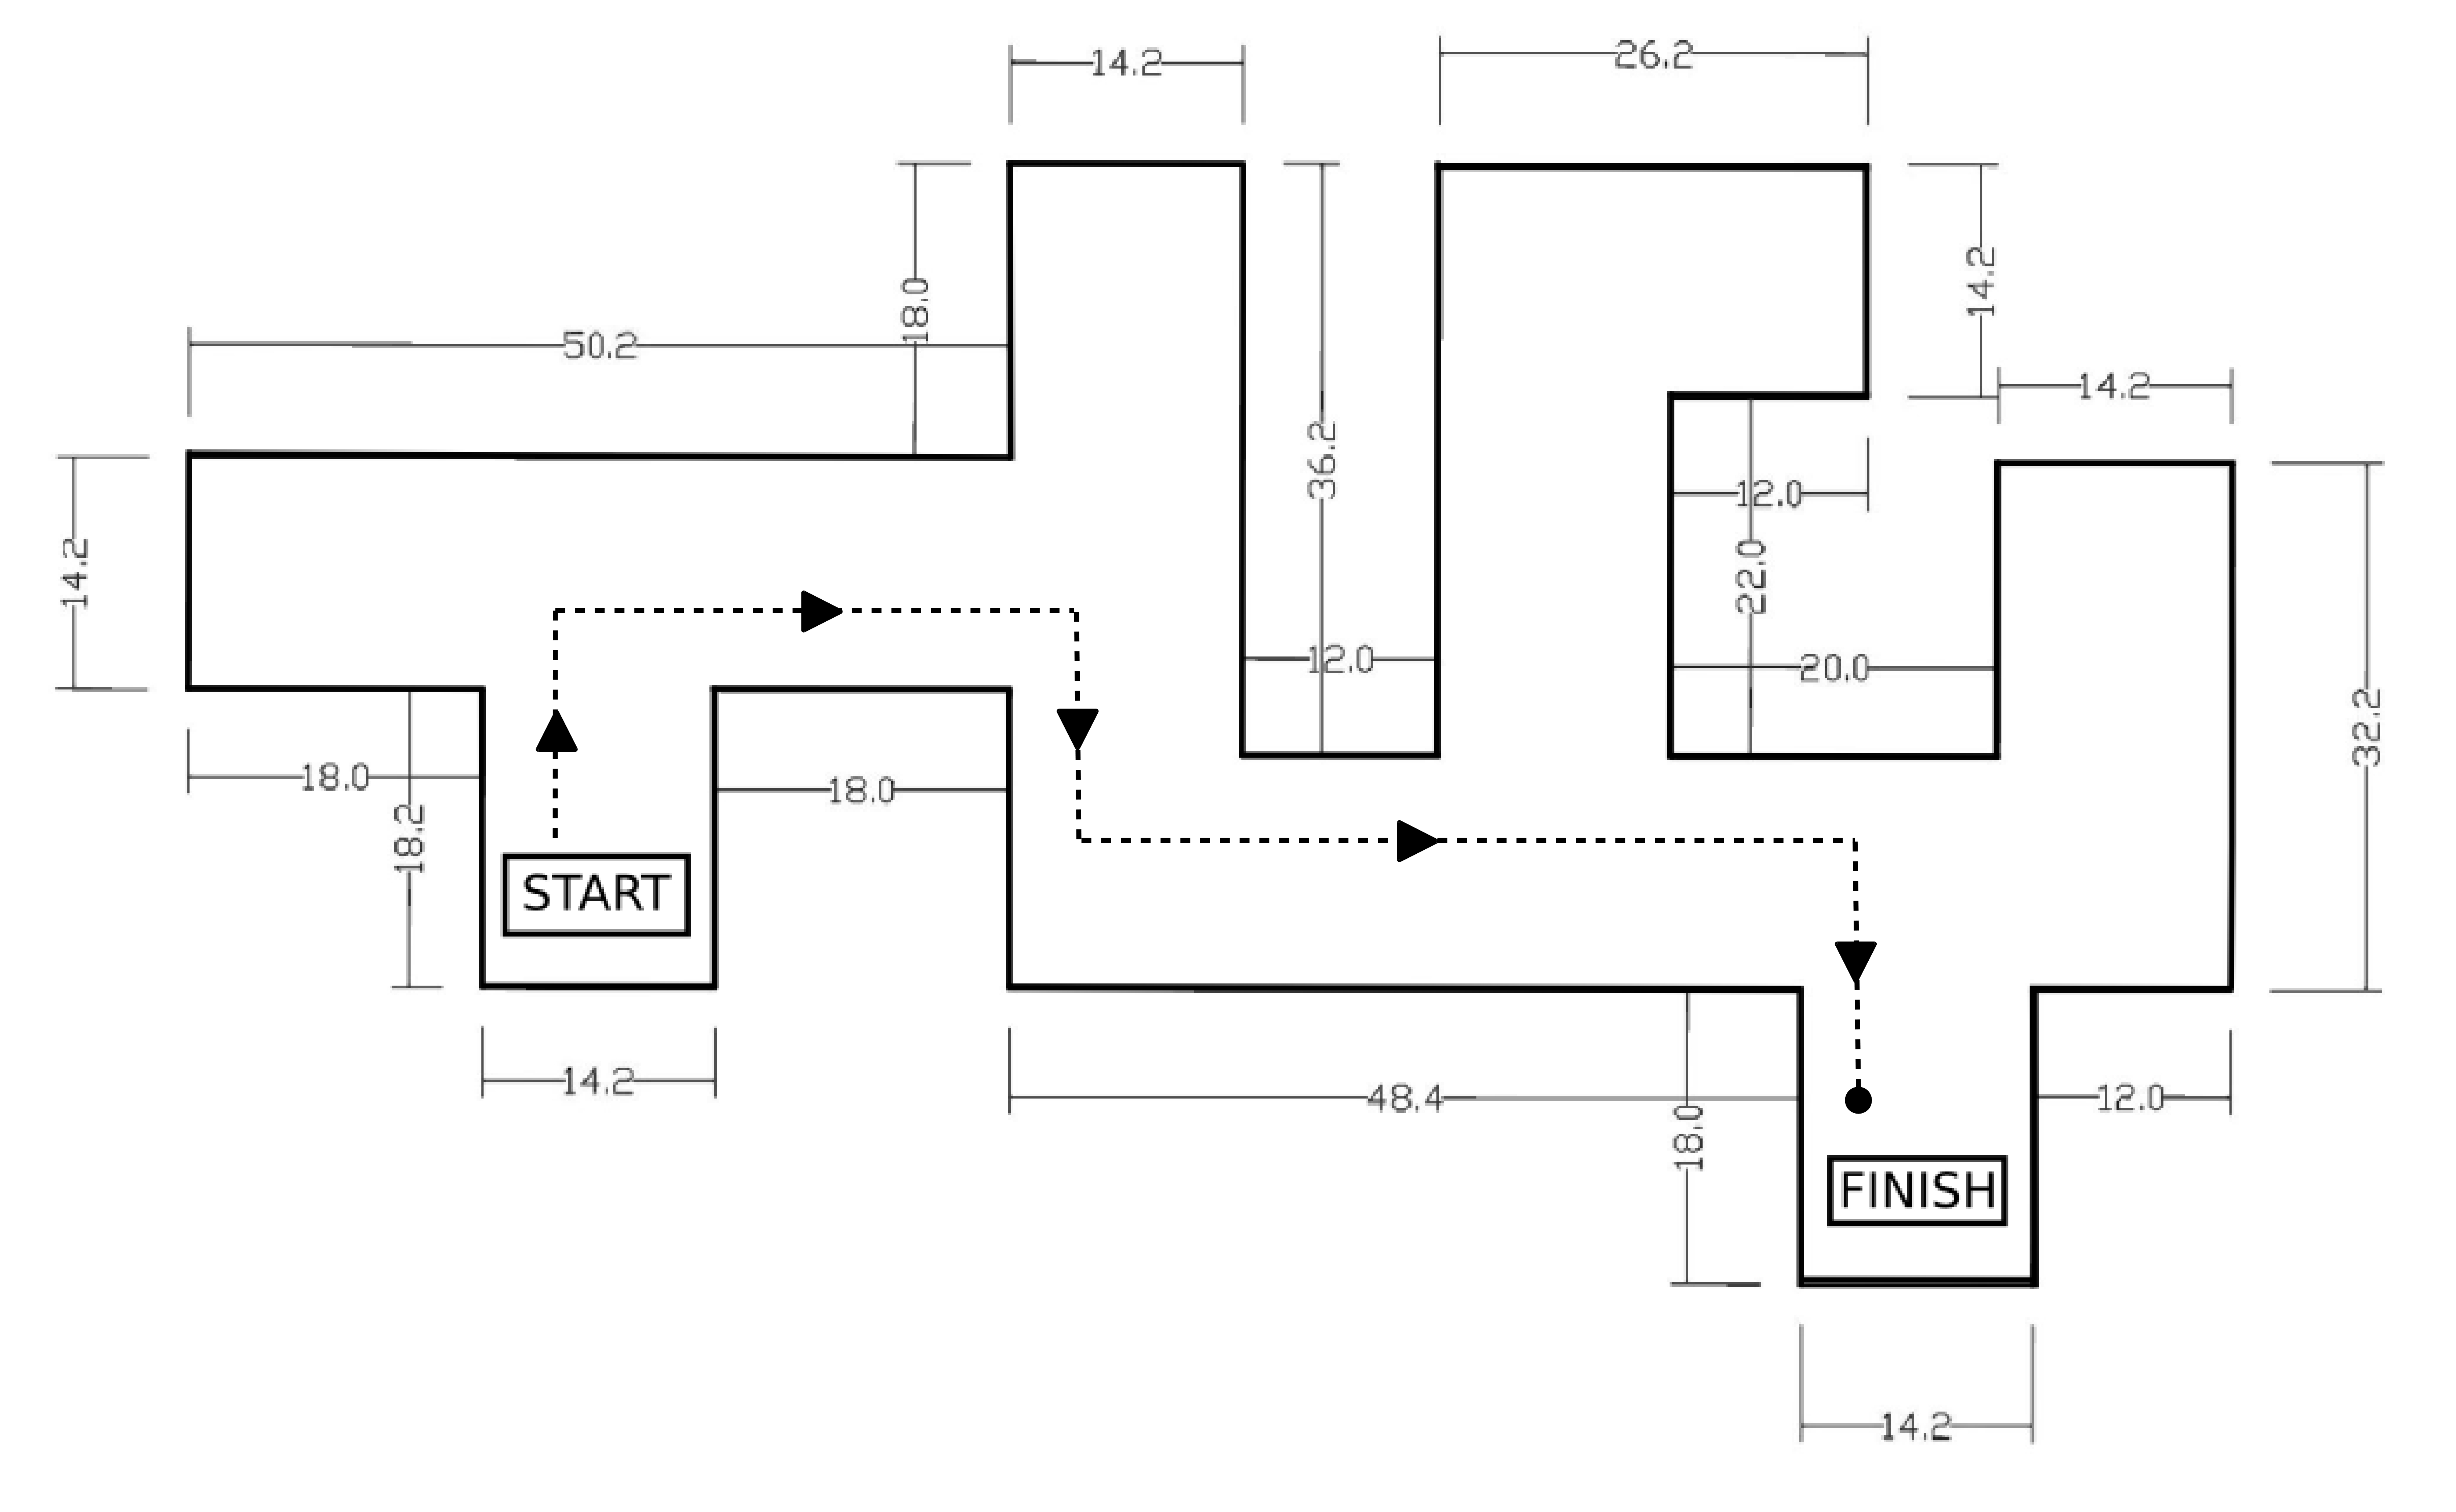
\includegraphics[scale=0.067]{mazetraverse_shortest_newnew.jpg} 
\caption{The shortest path followed by the second robot}
\end{figure}
%\subsection{PWM waveforms}
%For generating PWM waveforms, analogWrite function was used in the ATMEGA 328P microcontroller. It was then interfaced with H-Bridge to control the direction. By changing the direction of current flow in H-Bridge and interfacing it with Arduino, we have moved the robot in left, right, clockwise, anticlockwise and stopped it.  The motor was then connected with H-Bridge to change its direction. We have used pins 8, 9 ,6 and 5 of Arduino with IN1, IN2, IN3 and IN4 respectively of H-Bridge. The PWM waves were generated from  ENA (pin 10) and ENB (pin 9 ) of Motor 1 and 2 respectively.
%\begin{enumerate}
%\item When robot moved in clockwise direction
%\begin{figure}[h]
%\center
%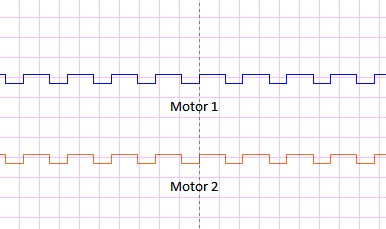
\includegraphics[scale=1]{pwm1_invert.jpg} 
%\caption{Waveforms of moor 1 and motor 2 in the clockwise direction}
%\end{figure}
%\item When robot moved in anti-clockwise direction
%\begin{figure}[h]
%\center
%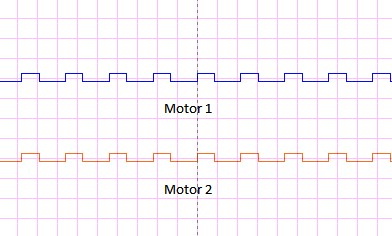
\includegraphics[scale=1]{pwm2_invert.jpg} 
%\caption{Waveforms of motor 1 and motor 2 in the anticlockwise direction}
%\end{figure}
%\item When motor moved in left direction
%\begin{figure}[h]
%\center
% 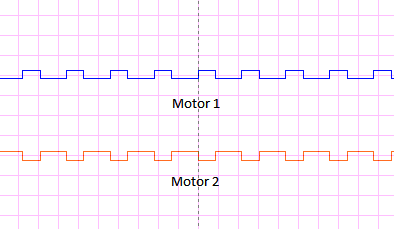
\includegraphics[scale=1]{leftd.png} 
%\caption{Waveforms of motor 1 and motor 2 in the left direction}
%\end{figure}
%\item When motor moved in right direction
%\begin{figure}[h]
%\center
%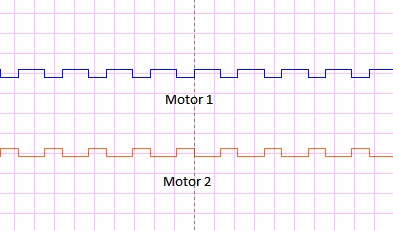
\includegraphics[scale=1]{rightd.png}   
%\caption{Waveforms of motor 1 and motor 2 in the right direction}
%\end{figure}
%\item When motor stopped\\
% For stopping the motor, all pins were set low, i.e, all IN1, IN2, IN3 and IN4 were 0. As all the pins were low so, no current was flown through the motor. No PWM value was given preventing the appearance of PWM waves.
%\end{enumerate}